\documentclass[compress, ucs, xelatex, 11pt, xcolor=x11names, aspectratio=1609,
	hyperref={
		bookmarks=true,
		unicode=true,
		colorlinks=true,
		pdftitle={HybSeq course},
		plainpages=false,
		pdfauthor={Vojtech Zeisek},
		pdfsubject={Practical processing of HybSeq target enrichment sequencing data on computing grids like MetaCentrum},
		pdfcreator={XeLaTeX},
		pdfkeywords={BASH, command line, GNU, HybSeq, Linux, MetaCentrum, sequencing shell, target enrichment},
		linkcolor=Cyan2, % Navigation menu links on pages and in navigation menus
		anchorcolor=Firebrick2, % Not in use?
		citecolor=Firebrick2, % Not in use?
		filecolor=Firebrick2, % Not in use?
		menucolor=Firebrick2, % Not in use?
		urlcolor=Chartreuse2, % Links with \href and \url
		pdftex},
	url={hyphens, lowtilde} % Allow line breaks within URLs
	]{beamer}

% Theme settings
\useoutertheme{infolines}
\useinnertheme[shadow]{rounded}
\usecolortheme{beetle}
% Headline
\setbeamertemplate{headline} {
	\begin{beamercolorbox}{section in head/foot}
		\insertsectionnavigationhorizontal{\paperwidth}{\hskip0pt plus1fill}{\hskip0pt plus1fill}
	\end{beamercolorbox}
	\begin{beamercolorbox}[ht=2ex, dp=1.125ex]{subsection in head/foot}
		\insertsubsectionnavigationhorizontal{\paperwidth}{}{\hfill\hfill}
	\end{beamercolorbox}
	}
% Color background for titles
\setbeamercolor{titlelike}{parent=palette secondary}

% Background for block titles
\setbeamercolor{block title}{bg=beetle@other}
\setbeamercolor{block title alerted}{bg=beetle@other}
\setbeamercolor{block title example}{bg=beetle@other}

% Fonts Linux Libertine
\usepackage{libertine}

% % Other packages
% \usepackage{multicol}
% \usepackage{tabularx}

% TeX logos
\usepackage{dtk-logos}

% % In-line higlighting
\renewcommand{\texttt}[1]{\colorbox{Snow4}{{\ttfamily #1}}}

% Change text color of highlighted text
\renewcommand{\alert}[1]{\textcolor{OrangeRed2}{#1}}

% Syntax higlight
\usepackage{minted}
\usemintedstyle{vim} % Styles are listed by pygmentize -L styles; languages are listed by pygmentize -L lexers
\newminted{bash}{linenos, fontsize=\footnotesize, bgcolor=Snow4, fontfamily=tt, gobble=4, numbersep=-3pt}
\newminted{splus}{linenos, fontsize=\footnotesize, bgcolor=Snow4, fontfamily=tt, gobble=4, numbersep=-3pt}
% Change line number style
\renewcommand{\theFancyVerbLine}{
	\sffamily
	\textcolor{DarkOrchid4}{
		\tiny
		\oldstylenums{
			\arabic{FancyVerbLine}
			}
		}
	}

% Fixing space before and after block of code higlight
\BeforeBeginEnvironment{bashcode}{\vspace{-0.5em}}
\AfterEndEnvironment{bashcode}{\par\vspace{-0.5em}}
\BeforeBeginEnvironment{spluscode}{\vspace{-0.5em}}
\AfterEndEnvironment{spluscode}{\par\vspace{-0.5em}}

% % Fixing space before and after multicols region
% \BeforeBeginEnvironment{multicols}{\vspace{-0.5em}}
% \AfterEndEnvironment{multicols}{\par\vspace{-0.5em}}

% Fixing space before and after itemize region
\BeforeBeginEnvironment{itemize}{\vspace{-0.25em}}
\AfterEndEnvironment{itemize}{\vspace{-0.25em}}

% Default language
\usepackage[main=american]{babel}

% Quotes
	\usepackage[autostyle=true, english=american]{csquotes}

% Title page
\author[Vojtěch Zeisek]{Vojtěch Zeisek, Roswitha Elisabeth Schmickl and Tomáš Fér}
\institute[\url{https://trapa.cz/}]{Department of Botany, Faculty of Science, Charles University, Prague\\Institute of Botany, Czech Academy of Sciences, Průhonice\\\url{https://trapa.cz/}, \href{mailto:zeisek@natur.cuni.cz}{zeisek@natur.cuni.cz}}
\title{HybSeq course}
\subtitle{Practical processing of HybSeq target enrichment sequencing data on computing grids like MetaCentrum}
\titlegraphic{
\includegraphics[width=1.5cm]{konsole.png}}
\date{January 20 to 23, 2020}

\begin{document}

\begin{frame}
	\titlepage
\end{frame}

\begin{frame}[allowframebreaks]{Outline}
	\tableofcontents
\end{frame}

\section{Introduction}

\begin{frame}{Resources before we start}
	\begin{itemize}
		\item Course \href{https://github.com/V-Z/hybseq-course}{git} and information: \url{https://trapa.cz/en/hybseq-course-2020}
		\item Most of the work is done in Linux/UNIX (macOS,~\ldots) command line, so that good knowledge of work in command line is essential, good starting point can be my Linux and MetaCentrum course \url{https://soubory.trapa.cz/linuxcourse/}
		\item Many tasks are done in R, so that at least basic knowledge of R is needed, good starting point can be my R course \url{https://soubory.trapa.cz/rcourse/}
		\item As \href{https://github.com/mossmatters/HybPiper/wiki}{HybPiper} is written in \href{https://www.python.org/}{Python}, so that at least minimal knowledge of this language is advantageous
		\item Processing HybSeq data is computationally demanding (it requires plenty of resources), during the course we use \href{https://www.metacentrum.cz/en/Sluzby/Grid/}{MetaCentrum, Czech National Grid Infrastructure} (slide~\ref{CESNET}), but any computing cluster or powerful desktop (for patient users;-) can be used
	\end{itemize}
\end{frame}

\begin{frame}{HybSeq and its data}
	\begin{itemize}
		\item \href{https://bsapubs.onlinelibrary.wiley.com/doi/full/10.3732/apps.1400042}{HybSeq} combines target enrichment and genome skimming (see lesson by RS) and especially in lager plant genomes it allows to select only $\sim$1000 single/low copy genes
		\item It requires sequencing probes, general or group specific (can be design using pipelines like \href{https://github.com/V-Z/sondovac/wiki}{Sondovač})
		\item From sequencing laboratory we get demultiplexed raw FASTQ files
		\item Steps leading to lists of gene trees require plenty of computing resources and disk space
		\begin{itemize}
			\item Even simple operation can take significant time --- think twice before every step
			\item User can select how much resources provide for each step --- depends on data size and available resources (more resources like CPU and memory will speed up processing)
		\end{itemize}
	\end{itemize}
\end{frame}

\subsection{Test data}

\begin{frame}{\textit{Oxalis} test data set}
	\begin{itemize}
		\item Genus \textit{Oxalis} has altogether ca. 500 species, over 200 in South Africa
		\item We selected 24 South African species (following \href{https://onlinelibrary.wiley.com/doi/full/10.1111/1755-0998.12487}{Schmickl et al. 2016}) as test data
		\item The probes used for sequencing were introduced in \href{https://onlinelibrary.wiley.com/doi/full/10.1111/1755-0998.12487}{Schmickl et al. 2016}, but were reduced (some probes with poor sequencing results were removed)
		\item For data structure see slide~\ref{datastructure}
		\item If you did not yet do so, download data (slide~\ref{datadownload}) --- it can take long time\ldots
	\end{itemize}
	\vfill
	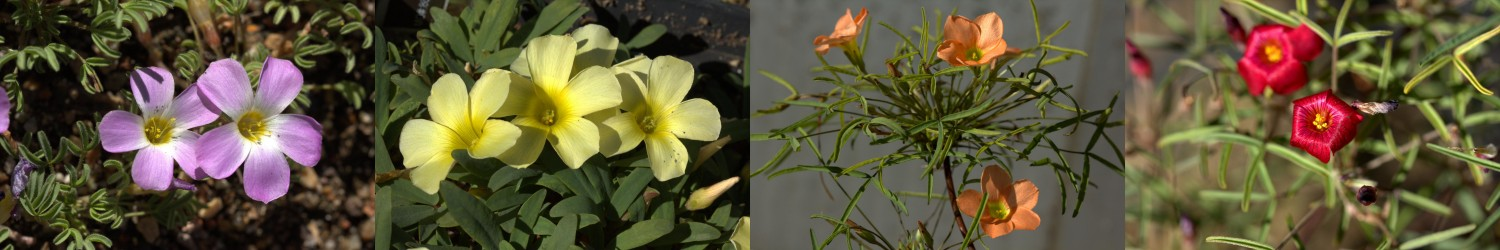
\includegraphics[width=\textwidth]{oxalis.jpg}
\end{frame}

\subsection{Data processing overview}

\begin{frame}[allowframebreaks]{Steps from sequencing files to species trees}
	\begin{enumerate}
		\item Trimming of raw sequencing FASTQ files (removal of adaptors,~\ldots) e.g. by \href{http://www.usadellab.org/cms/?page=trimmomatic}{Trimmomatic}
		\item Deduplication of FASTQ reads e.g. by \href{https://sourceforge.net/projects/bbmap/}{BBMap}
		\begin{itemize}
			\item Not strictly required, duplicates mainly provide wrong insight into real coverage of particular loci
		\end{itemize}
		\item Checking of FASTQ files in \href{https://www.bioinformatics.babraham.ac.uk/projects/fastqc/}{FastQC} or similar tool and removal of low-quality files
		\item Preparing probe reference FASTA file and list of samples for processing by HybPiper
		\item Processing every sample with with \href{https://github.com/mossmatters/HybPiper/wiki}{HybPiper} (or alternatively \href{https://github.com/tomas-fer/HybPhyloMaker}{HybPhyloMaker} or similar tool)
		\begin{enumerate}
			\item Mapping of FASTQ reads with \href{https://github.com/lh3/bwa}{BWA} to FASTA reference
			\item Distributing (sorting) of reads according to successful hits (using \href{https://github.com/samtools/samtools}{Samtools}) into FASTA files for assembly
			\item Assembly of sorted reads with \href{https://github.com/ablab/spades}{SPAdes}
			\item Alignment of SPAdes contigs against the target sequence
			\begin{itemize}
				\item Contigs are not expected to overlap much
				\item Initial exonerate search is filtered for hits that are above a certain threshold
				\item Contigs that pass this filter are arranged in order along the alignment
				\item All contigs that pass the previous steps are concatenated into a \enquote{supercontig} and the exonerate search is repeated
			\end{itemize}
			\item Search for paralogs --- if SPAdes assembler generates multiple contigs that contain coding sequences representing 75\% of the length of the reference protein, HybPiper will print a warning for that gene
			\item Recovering of the individual sequences
			\item Statistics of the recovery
			\item Cleanup of temporal files (especially SPAdes produces huge amount of data unneeded for further processing)
		\end{enumerate}
		\item Statistics of sequence lengths in all samples and more information about recovered contigs
		\item Creation of heatmaps (using \href{https://www.r-project.org/}{R} and packages \href{https://cran.r-project.org/package=gplots}{gplots} and \href{https://cran.r-project.org/package=heatmap.plus}{heatmap.plus}, or \href{https://cran.r-project.org/package=ggplot2}{ggplot2} and \href{https://cran.r-project.org/package=reshape2}{reshape2})
		\item Retrieve of sequences of exons, introns and supercontigs for all samples
		\item Alignment of all contigs (e.g. by \href{https://mafft.cbrc.jp/alignment/software/}{MAFFT}; or \href{https://www.drive5.com/muscle/}{MUSCLE}, \href{http://www.clustal.org/}{Clustal},~\ldots{ }e.g. using \href{https://www.r-project.org/}{R} and packages \href{https://cran.r-project.org/package=ape}{ape} and/or \href{https://cran.r-project.org/package=ips}{ips})
		\begin{itemize}
			\item All alignments must be trimmed --- columns/rows with too much missing data (e.g. beginning and end of the alignment) must be removed (e.g. using \href{https://www.r-project.org/}{R} and package \href{https://cran.r-project.org/package=ape}{ape})
			\item It is also useful to create simple NJ tree graphical check of alignment (e.g. using \href{https://www.r-project.org/}{R} and package \href{https://cran.r-project.org/package=ape}{ape})
		\end{itemize}
		\item Sorting of alignments, statistics of their length and quality, discarding of poor (too short, too few individuals, too few variable positions,~\ldots) alignments
		\item Reconstruction of gene trees from all aligned contigs (e.g. using \href{http://www.iqtree.org/}{IQ-TREE}, or \href{https://github.com/stamatak/ExaML}{ExaML}, \href{https://nbisweden.github.io/MrBayes/}{MrBayes}, \href{http://www.atgc-montpellier.fr/phyml/}{PhyML}, \href{https://github.com/stamatak/standard-RAxML}{RAxML},~\ldots)
		\item Post-processing of gene trees
		\begin{itemize}
			\item Identification, inspection and possible removal of gene trees with significantly different topology (e.g. by \href{https://www.r-project.org/}{R} and packages \href{https://cran.r-project.org/package=ape}{ape} and \href{https://cran.r-project.org/package=kdetrees}{kdetrees}, \href{https://github.com/uym2/TreeShrink}{TreeShrink})
			\item Comparison of gene trees (e.g. heatmaps and PCA by \href{https://www.r-project.org/}{R} and packages \href{https://cran.r-project.org/package=ade4}{ade4}, \href{https://cran.r-project.org/package=ape}{ape}, \href{https://cran.r-project.org/package=distory}{distory}, \href{https://cran.r-project.org/package=phytools}{phytools})
			\item Comparison of (several) (species) trees (e.g.by \href{https://www.r-project.org/}{R} and packages \href{https://cran.r-project.org/package=ape}{ape} or \href{https://cran.r-project.org/package=phytools}{phytools})
		\end{itemize}
		\item Construction of species trees (e.g. by \href{https://github.com/smirarab/ASTRAL}{ASTRAL})
		\begin{itemize}
			\item Comparison of species tree and gene trees (e.g. by \href{https://bitbucket.org/blackrim/phyparts}{phyparts} and \href{https://github.com/mossmatters/MJPythonNotebooks}{MJPythonNotebooks})
		\end{itemize}
		\item Phylogenetic networks (e.g. by \href{https://bioinfocs.rice.edu/PhyloNet}{PhyloNet})
	\end{enumerate}
	\vfil
	\begin{itemize}
		\item This general scheme can be significantly altered\ldots
		\item There are plenty of technical as well as biological problems (HGT, ILS,~\ldots) and new software keep being developed\ldots
		\item Much more analysis possible\ldots
	\end{itemize}
\end{frame}

\subsection{Software needed}

\begin{frame}[allowframebreaks]{List of software used during the course}
	\begin{itemize}
		\item \href{https://github.com/smirarab/ASTRAL}{ASTRAL} (see lesson by TF) --- species trees from gene trees
		\item BASH 4 or later and GNU core utils (\enquote{Linux command line})
		\item \href{https://sourceforge.net/projects/bbmap/}{BBMap} --- deduplication of FASTQ
		\item \href{ftp://ftp.ncbi.nlm.nih.gov/blast/executables/blast+/}{BLAST+} (used by \href{https://github.com/mossmatters/HybPiper/wiki}{HybPiper})
		\item \href{https://github.com/lh3/bwa}{BWA} (used by \href{https://github.com/mossmatters/HybPiper/wiki}{HybPiper})
		\item \href{https://www.ebi.ac.uk/about/vertebrate-genomics/software/exonerate}{Exonerate} (used by \href{https://github.com/mossmatters/HybPiper/wiki}{HybPiper})
		\item \href{https://www.gnu.org/software/parallel/}{GNU Parallel} (used by \href{https://github.com/mossmatters/HybPiper/wiki}{HybPiper} and in BASH scripts)
		\item \href{https://github.com/mossmatters/HybPiper/wiki}{HybPiper} --- recovering genes from targeted sequence capture data
		\item \href{http://www.iqtree.org/}{IQ-TREE} --- gene trees
		\item \href{https://mafft.cbrc.jp/alignment/software/}{MAFFT} --- alignment
		\item \href{https://github.com/mossmatters/MJPythonNotebooks}{MJPythonNotebooks} (used by \href{https://bitbucket.org/blackrim/phyparts}{phyparts})
		\item \href{https://bioinfocs.rice.edu/PhyloNet}{PhyloNet} --- phylogenetic networks
		\item \href{https://bitbucket.org/blackrim/phyparts}{phyparts} --- comparison of species tree vs. gene trees
		\item \href{https://www.python.org/}{Python 2.7 or later} and \href{https://biopython.org/}{Biopython 1.59 or later} (used by \href{https://github.com/mossmatters/HybPiper/wiki}{HybPiper})
		\item \href{https://github.com/lutteropp/QuartetScores}{QuartetScores} (see lesson by TF) --- support scores for internodes
		\item \href{https://www.r-project.org/}{R 3.5 or later} and packages \href{https://cran.r-project.org/package=ade4}{ade4}, \href{https://cran.r-project.org/package=adegenet}{adegenet}, \href{https://cran.r-project.org/package=ape}{ape}, \href{https://cran.r-project.org/package=corrplot}{corrplot}, \href{https://cran.r-project.org/package=distory}{distory}, \href{https://cran.r-project.org/package=ggplot2}{ggplot2}, \href{https://cran.r-project.org/package=gplots}{gplots}, \href{https://cran.r-project.org/package=heatmap.plus}{heatmap.plus}, \href{https://cran.r-project.org/package=ips}{ips}, \href{https://cran.r-project.org/package=kdetrees}{kdetrees}, \href{https://cran.r-project.org/package=pegas}{pegas}, \href{https://cran.r-project.org/package=phangorn}{phangorn}, \href{https://cran.r-project.org/package=phytools}{phytools} and \href{https://cran.r-project.org/package=reshape2}{reshape2}
		\begin{itemize}
			\item Used by \href{https://github.com/mossmatters/HybPiper/wiki}{HybPiper}, for alignment of contigs, post-processing of alignments, post-processing and comparison of gene trees, etc.
		\end{itemize}
		\item \href{https://github.com/samtools/samtools}{Samtools} (used by \href{https://github.com/mossmatters/HybPiper/wiki}{HybPiper})
		\item \href{https://github.com/ablab/spades}{SPAdes} (used by \href{https://github.com/mossmatters/HybPiper/wiki}{HybPiper})
		\item \href{https://github.com/uym2/TreeShrink}{TreeShrink} --- detection of outlier long branches in collections of phylogenetic trees
		\item \href{http://www.usadellab.org/cms/?page=trimmomatic}{Trimmomatic} --- trimming of FASTQ
	\end{itemize}
\end{frame}

\subsection{MetaCentrum computing environment}

\begin{frame}[allowframebreaks]{CESNET and MetaCentrum}
	\label{CESNET}
	\begin{itemize}
		\item \href{https://www.cesnet.cz/?lang=en}{CESNET} is organization of Czech universities, Academy of Science and other organizations taking care about Czech backbone Internet, one of world leading institutions of this type
		\item CESNET provides various \href{https://www.cesnet.cz/services/?lang=en}{services}
		\begin{itemize}
			\item Massive computations --- \href{https://www.cesnet.cz/services/massive-computations-metacentrum/?lang=en}{MetaCentrum} --- \alert{this we need to process our HybSeq data}
			\item Large \href{https://www.cesnet.cz/services/data-storage/?lang=en}{data storage} --- \alert{this we need to store our HybSeq data}
			\item \href{https://www.cesnet.cz/services/filesender/?lang=en}{FileSender} to be able to send up to 1.9~TB file
			\item \href{https://www.metacentrum.cz/en/Sluzby/Cloud/}{Cloud} --- computing (HPC) cloud similar to e.g. Amazon Elastic Compute Cloud (EC2) or Google Compute Engine
			\item \href{https://www.cesnet.cz/services/owncloud/?lang=en}{ownCloud} to backup and/or sync data across devices (default capacity is 100~GB, user may ask for more) --- similar to e.g. Dropbox
			\begin{itemize}
				\item It is possible to connect by webDAV to ownCloud--- many applications support it
				\item It is possible to share calendars and/or address books via calDav and cardDav among devices and/or people
			\end{itemize}
		\end{itemize}
		\item Services accessible without registration
		\begin{itemize}
			\item ownCloud \url{https://owncloud.cesnet.cz/}
			\item FileSender \url{https://filesender.cesnet.cz/}
			\item Go to web and log in with your institutional password
		\end{itemize}
		\item Services requiring registration (and approval)
		\begin{itemize}
			\item To use MetaCentrum fill registration form \url{https://metavo.metacentrum.cz/en/application/form}
			\item To use data storage fill registration form \url{https://einfra.cesnet.cz/perun-registrar-fed/?vo=storage}
			\item After registration for MetaCentrum, user can join MetaCloud via \url{https://perun.metacentrum.cz/fed/registrar/?vo=meta&group=metacloud}
			\item Users not having access to \href{https://www.eduid.cz/en/index}{EduID} have to register first at HostelID \url{http://hostel.eduid.cz/en/index.html}
		\end{itemize}
		\item Information about data storage \url{https://du.cesnet.cz/en/start} contains detailed usage instructions
		\item Information about MetaCentrum \url{https://www.metacentrum.cz/en/}
		\item Information about MetaCloud \url{https://wiki.metacentrum.cz/wiki/Kategorie:Clouds}
		\item Most of practical information for users are at wiki \url{https://wiki.metacentrum.cz/w/index.php?&setlang=en}
	\end{itemize}
	\begin{alertblock}{MetaCentrum vs. other clusters\ldots}
		I show processing on MetaCentrum Czech National Grid Infrastructure, as it is readily available, well maintained and contains all needed applications, but it's possible to use any computing cluster in similar way.
	\end{alertblock}

\end{frame}

\begin{frame}{MetaCentrum}
	\begin{itemize}
		\item Find all needed information at \url{https://wiki.metacentrum.cz/wiki/Main_Page}
		\item Current state and usage as available at \url{https://metavo.metacentrum.cz/en/}
		\item Manage your user account at \url{http://metavo.metacentrum.cz/en/myaccount/}
		\item Personal view on actual resources and running tasks is at \url{https://metavo.metacentrum.cz/pbsmon2/person}
		\item List of available applications \url{https://wiki.metacentrum.cz/wiki/Kategorie:Applications}
		\item It has 9~\href{https://wiki.metacentrum.cz/wiki/Frontend}{frontends} where users log and thousands of computers doing the calculations --- they are not accessed directly to run task
		\item Most of computers are running \href{https://www.debian.org/}{Debian GNU/Linux}
	\end{itemize}
\end{frame}

\begin{frame}[fragile]{MetaCentrum usage}
	\begin{itemize}
		\item User can transfer data on one of \href{https://wiki.metacentrum.cz/wiki/Frontend}{frontends} or to \href{https://du.cesnet.cz/en/prehled_protokolu_a_sluzeb_s_jejich_doporucenimi/start#protocol}{data storage} by e.g. \texttt{scp} or \href{https://winscp.net/}{WinSCP} from Windows or \href{https://filezilla-project.org/}{FileZilla} from anywhere
		\item Same credentials are used for all frontends, computing nodes as well as data storage, for SSH login as well as file transmissions
	\end{itemize}
	\vfill
	\begin{bashcode}
    # Login to selected server (tarkil is located in Prague)
    ssh USER@tarkil.metacentrum.cz
    # Continue as in any other command line...
    qsub ... # Submit the job (see later)
	\end{bashcode}
	\vfill
	\begin{itemize}
		\item In home directory on the server prepare all needed data and non-interactive script (interactive are more complicated) which will do the calculations
		\item Tasks are not launched immediately, but using \texttt{qsub} the task is submitted into queue and system decides when it will be launched
	\end{itemize}
\end{frame}

\begin{frame}{File transfers to MetaCentrum}
	\begin{itemize}
		\item Graphical applications: \href{https://winscp.net/}{WinSCP}, \href{https://filezilla-project.org/}{FileZilla} or from most of file managers
		\item Protocol is SSH/SSH2/SFTP/SCP, port 22, server is selected \href{https://wiki.metacentrum.cz/wiki/Frontend}{frontend's} address (e.g. \texttt{tarkil.metacentrum.cz}) --- it is recommendable to use all the time same frontend
		\item All servers are accessible under domain \texttt{*.metacentrum.cz}: \texttt{skirit}, \texttt{perian}, \texttt{onyx}, \texttt{zuphux} (located in Brno), \texttt{alfrid}, \texttt{nympha}, \texttt{minos} (in Pilsen), \texttt{tarkil} (in Prague), and \texttt{tilia} (in Průhonice) --- so that e.g. \texttt{tarkil.grid.cesnet.cz} is synonymous to \texttt{tarkil.metacentrum.cz}
		\item In the same way use SCP/SFTP/rsync/SSH to \texttt{ssh.du4.cesnet.cz} to access the storage, see \href{https://du.cesnet.cz/en/prehled_protokolu_a_sluzeb_s_jejich_doporucenimi/start\#protocol}{help}
	\end{itemize}
\end{frame}

\begin{frame}[fragile]{Launching of tasks}
	\begin{itemize}
		\item \url{https://wiki.metacentrum.cz/wiki/How_to_compute/Requesting_resources}
		\item Personal view \url{https://metavo.metacentrum.cz/pbsmon2/person} has nice overview of available resources and tasks and allows comfortable construction of submission command
	\end{itemize}
	\vfill
	\begin{bashcode}
    # We will run up to 5 days (120 h), require one physical
    # computer with 8 CPU threads, 24 GB of RAM, 10 GB of disk
    # space and we get all information mails
    qsub -l walltime=120:0:0 -l select=1:ncpus=8:mem=24gb:
      scratch_local=10gb -m abe metacentrum.sh
    # Check how the task is running (above web) and
    qstat -u $USER # Information about $USER's jobs
    qstat 123456789 # The task ID is available from qstat
    qstat -f 123456789 # Print a lot of details
    qdel 123456789 # Terminate scheduled or running task
	\end{bashcode}
\end{frame}

\begin{frame}[fragile]{Key MetaCentrum commands}
	\begin{itemize}
		\item MetaCentrum is \enquote{just} normal Linux server --- work as usually
		\item Command \texttt{module} loads/unloads selected \href{https://wiki.metacentrum.cz/wiki/Kategorie:Applications}{application}
		\item Tasks (BASH scripts) are submitted for computing by \texttt{qsub} --- the script must copy the data into \texttt{\$SCRATCHDIR} and do all calculations there
		\begin{itemize}
			\item It has plenty of options how to specify requirements (see \href{https://wiki.metacentrum.cz/wiki/About_scheduling_system}{help})
		\end{itemize}
		\item Queued and running jobs can be seen by \texttt{qstat -u \$USER} (\texttt{qstat} has much more options) and any job can be terminated by \texttt{qdel 123456789} (number from \texttt{qstat})
	\end{itemize}
	\vfill
	\begin{bashcode}
    module add <TAB><TAB> # Load some module
    module rm XXX # Unload selected module
    module list # List of currently loaded modules
    qsub ... # Submit task for computing
    qstat -u $USER # See $USER's running and queued jobs
    qdel 123456789 # Termite task (number from qstat)
	\end{bashcode}
\end{frame}

\begin{frame}[allowframebreaks]{Scheduling details}
	\begin{itemize}
		\item Specify needed time
		\begin{itemize}
			\item Always \texttt{hours:minutes:seconds}, so e.g. for 4~weeks use -\texttt{l~walltime=672:0:0} (28~$\cdot$~24), for two days and 12 hours -\texttt{l~walltime=60:0:0}
			\item User \href{mailto:meta@cesnet.cz}{may ask} to prolong the walltime --- it is needed to write in advance
		\end{itemize}
		\item Ask for as much RAM as you need (e.g. -\texttt{l~mem=8gb} to request 8~GB of memory)
		\begin{itemize}
			\item If the task is going to require more, than allowed, system kills it\ldots
			\item If user doesn't use all required RAM, the system temporarily lowers priority for future tasks
			\item It can be hard to estimate\ldots
		\end{itemize}
		\item Disk space is relatively free resource, user can ask more to have some reserve (e.g. -\texttt{l~scratch\_local=10gb} to request 10~GB)
		\item Specify how many physical computer(s) you are going to use (e.g. -\texttt{l~select=1} for one machine) and number of CPU threads on each machine (e.g. -\texttt{l~select=1:ncpus=8} for 1~machine with 8~cores or -\texttt{l~select=2:ncpus=4} for 2~machines, each with 4~CPU threads)
		\begin{itemize}
			\item It use to be necessary to specify correct number of threads for the application (e.g. \texttt{parallel}~-\texttt{j 4}) --- the application sees all CPUs on the machine, but can't use them
			\item If the application consumes less than required, the system temporarily lowers priority for future tasks, if it try to use more, it will be very slowed down or killed by the server
		\end{itemize}
		\item If requesting e-mails (e.g. -\texttt{m abe} to get mail about abort, beginning and exit of the task) and submitting plenty of tasks by some script, it can result in hundreds of mails --- receiving mail servers don't like it\ldots
		\item Every user has certain \href{https://metavo.metacentrum.cz/pbsmon2/users/}{priority} highered by \href{https://wiki.metacentrum.cz/wiki/Usage_rules/Acknowledgement}{acknowledgments} in publications to MetaCentrum and lowered by intensive usage of the service (the usage is calculated from past month)
		\item After submission of the task, check in \href{https://metavo.metacentrum.cz/pbsmon2/queues/jobsQueued}{the queue} in which state it is --- sometimes it can't start because of impossible combination of resources or so
		\item User can \href{https://metavo.metacentrum.cz/pbsmon2/nodes/physical}{check load of machines}
		\item For more options read \url{https://wiki.metacentrum.cz/wiki/How_to_compute/Requesting_resources}
		\begin{itemize}
			\item Request special CPU (AMD, graphical,~\ldots), e.g. CPU with AVX2 -\texttt{l~select=cpu\_flag=avx2}
			\item Request particular location, ...
			\item \url{https://metavo.metacentrum.cz/pbsmon2/qsub_pbspro} helps with preparation of \texttt{qsub} command
		\end{itemize}
	\end{itemize}
\end{frame}

\begin{frame}[fragile]{Get to task's working directory}
	\begin{itemize}
		\item Go to \url{https://metavo.metacentrum.cz/pbsmon2/person} and click to list of your tasks and click to selected task
		\item Search for information \textbf{exec\_host} (address of node doing the task) and \textbf{SCRATCHDIR} (temporal directory for all data and results)
		\item Sometimes one needs to monitor task progress or influence it
		\item It is not possible to directly modify running task, but at least check (and possibly modify) input data and see outputs
	\end{itemize}
	\begin{bashcode}
    # From MetaCentrum frontend login to node running the task
    ssh exec_host # No need to specify user name; e.g. mandos9
    # Go to SCRATCH directory
    cd SCRATCHDIR # e.g. /scratch/gunnera/job_90220.meta-pbs...
    # There are working data of currently running task...
    # Check whatever you need...
	\end{bashcode}
\end{frame}

\begin{frame}{Running R tasks on MetaCentrum}
	\begin{itemize}
		\item There are no R packages, user must create local package library and provide path --- \alert{Be careful about paths!}
		\item In the \texttt{metacentrum.sh} script load R \texttt{module add R-3.5.1-gcc} and start R script as usually \texttt{R CMD BATCH script.r}
	\end{itemize}
	\begin{enumerate}
		\item Login to selected front node via SSH
		\item Go to working directory \texttt{cd workdir}
		\item Create new directory for R packages \texttt{mkdir rpkgs}
		\item Start R \texttt{R} and install \textbf{all} R packages needed for the task --- install them into the \texttt{rpkgs} directory: \texttt{install.packages(pkgs=..., lib="rpkgs")}
		\item In the R script load the packages from the \texttt{rpkgs} directory \texttt{library(package=..., lib.loc="rpkgs")}
		\item Ensure all needed outputs are saved from the R script
	\end{enumerate}
\end{frame}

\section{Data preprocessing}

\begin{frame}[fragile]{Data download}
	\label{datadownload}
	\begin{itemize}
		\item It's not possible to store such large data on MetaCentrum frontend, it must be download to the CESNET storage
		\item Servers powering CESNET storage have only very limited set of command line tools available
		\item We can login to any MetaCentrum frontend and then go to directory where the storage is accessible
	\end{itemize}
	\begin{bashcode}
    # Login to any MetaCentrum frontend
    ssh USER@tarkil.grid.cesnet.cz # Or any other fronted
    # Go to your directory on the CESNET data storage
    cd /storage/ostrava2-archive/tape_tape/backup/VO_storage/
      home/$USER/ # $USER's home on the storage
    # Download the course data
    wget ftp://botany.natur.cuni.cz/hybseq_course.zip
    # Unpack it
    unzip hybseq_course.zip
	\end{bashcode}
\end{frame}

\begin{frame}[fragile]{Scripts and other resources to process the data}
	\begin{itemize}
		\item The archive \texttt{hybseq\_course.zip} contains test data as well as needed scripts, R packages, HybSeq reference,~\ldots
		\item The other resources (not the data in the \texttt{oxalis} directory) should be moved to the frontend
		\item Inspect content of the \texttt{bin} and \texttt{hybseq} directories
		\item Scripts must be updated to point to correct location of the \texttt{oxalis}
	\end{itemize}
	\begin{alertblock}{Do not blindy copy-paste commands\ldots}
		\alert{Commands show typical way how to proceed, but should not be using without understanding, and onther ways how to work are possible\ldots}
	\end{alertblock}
	\begin{bashcode}
    # Login to any MetaCentrum frontend
    ssh USER@tarkil.grid.cesnet.cz # Or any other fronted
    # Move scripts and other resources into home directory
    mv /storage/ostrava2-archive/tape_tape/backup/VO_storage/
      home/$USER/{bin,hybseq} ~/ # Note $USER/{...,...} syntax
	\end{bashcode}
\end{frame}

\subsection{General data structure}

\begin{frame}[fragile]{\textit{Oxalis} test data directory structure I}
	\label{datastructure}
	\begin{bashcode}
    ├── bin # BASH script to be submitted by qsub
    │   └── HybPiper # HybPiper Python and R scripts
    ├── hybseq # BASH scripts to process the data
    │   ├── dedup # Output directory for deduplicated sequences
    │   ├── qual_rep # Output directory for FastQC reports
    │   ├── ref # References for HybPiper
    │   ├── rpackages # R library with installed R packages
    │   └── trimmed # Output directory for trimmed sequences
    └── oxalis # Oxalis test data
        ├── 1_data # Sequencing libraries
        │   ├── lib_01 # Sequencing library 1
        │   │   ├── 0_data # Raw FASTQ sequences
        │   │   ├── 1_trimmed # Trimmed FASTQ sequences
        │   │   ├── 2_dedup # Deduplicated FASTQ sequences
        │   │   └── 3_qual_rep # FastQC quality reports
        │   └── lib_02 # Sequencing library 2
        ... ... ├... # Next slide...
	\end{bashcode}
\end{frame}

\begin{frame}[fragile]{\textit{Oxalis} test data directory structure II}
	\begin{bashcode}
        ... ... ... # Previous slide...
        │   │   ├── 0_data # Raw FASTQ sequences
        │   │   ├── 1_trimmed # Trimmed FASTQ sequences
        │   │   ├── 2_dedup # Deduplicated FASTQ sequences
        │   │   └── 3_qual_rep # FastQC quality reports
        ├── 2_seqs # Outputs of HybPiper
        │   ├── o_amblyodonta_S524.dedup # Sample output dir
        │   │   ├── Assembly_10176 # Gene output directory
        │   │   ├── Assembly_10307 # Gene output directory
        │   │   ├── ... # Gene output directory
        │   ├── ... # More samples...
        │   └── o_zeekoevleyensis_S518.dedup # Sample output dir
        │   │   ├── Assembly_10176 # Gene output directory
        │   │   ├── Assembly_10307 # Gene output directory
        │   │   ├── ... # Gene output directory
        ├── 3_aligned # Aligned contigs
        ... ├... # Next slide...
	\end{bashcode}
\end{frame}

\begin{frame}[fragile]{\textit{Oxalis} test data directory structure III}
	\begin{bashcode}
        ... ... # Previous slide...
        │   ├── exons # Aligned exons
        │   ├── introns # Aligned introns
        │   └── supercontigs # Aligned supercontigs
        ├── 4_gene_trees # Reconstructed gene trees
        │   ├── exons # Gene trees of exons
        │   ├── introns # Gene trees of introns
        │   └── supercontigs # Gene trees of supercontigs
        └── 5_species_trees # Processing of the trees
            ├── distances_kdetrees_comparisons
            ├── phyparts # Comparison of species vs. gene trees
            ├── phylonet # Phylogenetic networks
            └── treeshrink # Identification of outlied branches
            ... # More downstream analysis...
	\end{bashcode}
	\begin{itemize}
		\item Of course, every user can figure different directory structure, but HybSeq produces a lot of data and plenty of software packages are used, so keep some logical structure\ldots
	\end{itemize}
\end{frame}

\subsection{Trimming and deduplication}

\begin{frame}{Trimming and deduplication}
	\begin{itemize}
		\item Raw demultiplexed FASTQ sequences must be trimmed (sequencing adaptors removed,~\ldots) and should be deduplicated (removal of artificial duplicates to get correct statistics of coverage)
		\item There are plenty of software packages available, \href{http://www.usadellab.org/cms/?page=trimmomatic}{Trimmomatic} use to be used for trimming and e.g. \href{https://sourceforge.net/projects/bbmap/}{BBMap} for deduplication
		\item Usually, libraries are processed as they are delivered from sequencing company
		\item Quality of all FASTQ files should be checked by e.g. \href{https://www.bioinformatics.babraham.ac.uk/projects/fastqc/}{FastQC}
		\item It is practical to obtain simple statistics --- number of sequences in original files, after trimming and after deduplication
		\item Low quality files should be discarded\ldots
		\item Everything can be easily coded into simple BASH script processing all files (see following slides)
	\end{itemize}
\end{frame}

\begin{frame}{Scripts to trim and deduplicate FASTQ sequences}
	\begin{itemize}
		\item Script \texttt{$\sim$/hybseq/hybseq\_1\_prep.sh}
		\begin{itemize}
			\item See \texttt{./hybseq\_run\_1\_prep.sh -h} for usage help
			\item Script checks if all needed parameters and tools are available and in simple \texttt{for} loop trimms all sequences (one by one), deduplicates them, does quality checking, prints simple statistics, and prepares list of samples for HybPiper
		\end{itemize}
		\item Script \texttt{$\sim$/bin/hybseq\_run\_1\_prep.sh}
		\begin{itemize}
			\item Submits via \texttt{qsub} script \texttt{$\sim$/bin/hybseq\_run\_1\_prep.sh} for calculation
			\item Variables \texttt{WORKDIR} and \texttt{DATADIR} must point to correct existing location
			\item The script is started twice to process both sequencing libraries
			\item If changing parameters for \texttt{hybseq\_1\_prep.sh}, parameters for \texttt{qsub} must be changed accordingly
		\end{itemize}
	\end{itemize}
\end{frame}

\begin{frame}[fragile]{Submission of hybseq\_1\_prep.sh}
	\begin{itemize}
		\item To prepare data for HybPiper
		\item \alert{\texttt{~/bin/hybseq\_run\_1\_prep.sh} must be edited before submission via \texttt{qsub}}
		\item After it runs for a while (everything had been copyied to the computing node), it is possible to change \texttt{DATADIR} and submit processing of the second library
	\end{itemize}
	\begin{bashcode}
    # After edition of WORKDIR and DATADIR run
    qsub -l walltime=12:0:0 -l select=1:ncpus=4:mem=16gb:
      scratch_local=100gb -m abe ~/bin/hybseq_run_1_prep.sh
    # Or similar command
    # Monitor running $USER's tasks with details
    qstat -w -n -1 -u $USER # Last column contains machine name
    # See your processes running the machine (from above list)
    ssh exec_node "ps ux" # Replace exec_host by hostname!
	\end{bashcode}
\end{frame}

\begin{frame}{Trimm and deduplicate all FASTQ files}
	\begin{exampleblock}{Tasks to pre-process FASTQ data for HybPiper}
			\begin{enumerate}
		\item Inspect \texttt{$\sim$/hybseq/hybseq\_1\_prep.sh} and \texttt{$\sim$/bin/hybseq\_run\_1\_prep.sh} be sure to understand what the scripts do, including syntax used.
		\item Edit declaration of variables \texttt{WORKDIR} and \texttt{DATADIR} so that they point to correct locations.
		\item Submit via \texttt{qsub} \texttt{$\sim$/bin/hybseq\_run\_1\_prep.sh} to process both libraries and monitor the jobs during processing.
		\item Inspect outputs of \texttt{$\sim$/bin/hybseq\_run\_1\_prep.sh}, including statistics and FASTQ checks. What do they show?
		\item Can you run the task on your computer (desktop in office or notebook) without \texttt{qsub}? If so, how?
		\end{enumerate}
	\end{exampleblock}
\end{frame}

\subsection{Preparing data for HybPiper}

\begin{frame}{Requirements to run HybPiper}
	\begin{itemize}
		\item See \url{https://github.com/mossmatters/HybPiper/} to see software requirements to run HybPiper
		\item It is possible to run HybPiper on your computer (with Linux or macOS), but it requires plenty of CPU and memory and creates huge output directories\ldots
		\item To process multiple files (by \texttt{while} loop or by \texttt{$\sim$/bin/hybseq\_run\_2\_hybpiper\_1\_submitter.sh}) there must be list of sample base names without suffixes like \texttt{*[.\_]R\{1,2\}.f*q*} (here created by \texttt{hybseq\_1\_prep.sh})
		\item Reference bait FASTA file \textbf{must} have sequences named as \texttt{Species\_name-gene\_id} (see \href{https://github.com/mossmatters/HybPiper/wiki\#target-file}{help}) (\alert{note} order and dash in between)
		\item \href{https://github.com/mossmatters/HybPiper}{HybPiper} is processing individual files with given baits FASTA sequences --- batch processing must be scripted
	\end{itemize}
\end{frame}

\begin{frame}{Before running HybPiper}
	\begin{itemize}
		\item Directory \texttt{$\sim$/hybseq/ref/} contains prepared reduced bait file \texttt{new\_soa\_probes\_gen\_comp.fasta} (it will be used to process test data) and unreduced \texttt{input\_seq\_without\_cpdna\_1086\_loci\_renamed.f\ldots} (with renamed sequences from \texttt{input\_seq\_without\_cpdna\_1086\_loci.fa})
		\item To run \href{https://github.com/mossmatters/HybPiper}{HybPiper} we need both files above and all required software, and BASH script to process all input files in batch --- see \texttt{hybseq\_run\_2\_hybpiper\_1\_submitter.sh} (submitting via \texttt{qsub} all input files), \texttt{hybseq\_run\_2\_hybpiper\_2\_qsub.sh} (preparing individual job to run) and \texttt{hybseq\_2\_hybpiper.sh} (processing every input file --- doing the job)
	\end{itemize}
\end{frame}

\begin{frame}{Prepare to run HybPiper}
	\begin{exampleblock}{Tasks before running HybPiper}
		\begin{enumerate}
			\item Check \texttt{samples\_list.txt} in \texttt{2\_dedup} output directories of both libraries after running \texttt{$\sim$/hybseq/hybseq\_1\_prep.sh}, and check how it was created.
			\item In \texttt{input\_seq\_without\_cpdna\_1086\_loci.fa} (output of Geneious assembler) consider \texttt{Contig\_\#} (\texttt{\#} stands for number) as standing for \texttt{Oxalis\_obtusa\_\#} (mutliple \textit{Oxalis obtusa} individuals were used) and \texttt{Assembly\_\#} as gene ID and think how to transfor it to form required by \href{https://github.com/mossmatters/HybPiper/wiki\#target-file}{HybPiper} (also discard final \texttt{\_\#}). Use any good text editor (or \texttt{sed} and another command line tools) and regular expressions.
			\item Do we have everyhting needed to run \href{https://github.com/mossmatters/HybPiper}{HybPiper}?
		\end{enumerate}
	\end{exampleblock}
\end{frame}

\section{HybPiper}

\begin{frame}{Overview of HybPiper}
	\begin{center}
		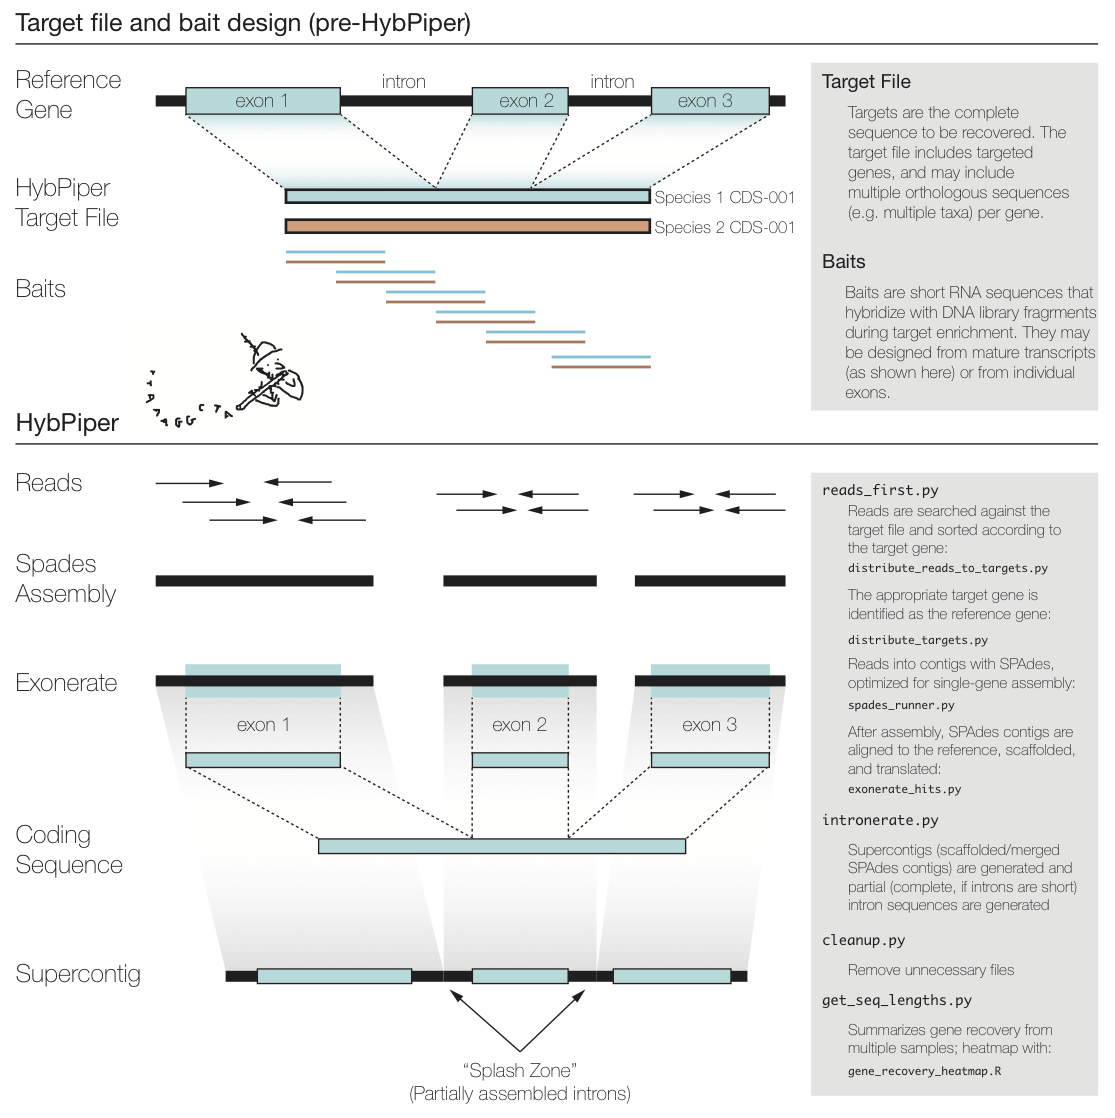
\includegraphics[height=7cm]{hybpiper.png}
	\end{center}
\end{frame}

\subsection{Processing input files}

\begin{frame}[allowframebreaks]{Understanding how presented scripts run HybPiper}
	\begin{itemize}
		\item Script \texttt{$\sim$/bin/hybseq\_run\_2\_hybpiper\_1\_submitter.sh} goes to directory set by \texttt{DATADIR} and for every sample (forward and reverse FASTQ files) listed in \texttt{samples\_list.txt} (variable \texttt{SAMPLES}, created by \texttt{hybseq\_2\_hybpiper.sh}) submits via \texttt{qsub} individual task
		\item Script \texttt{$\sim$/bin/hybseq\_run\_2\_hybpiper\_2\_qsub.sh} drives submission and manipulation of processing of each individual file --- it checks if all required data are provided, copy input files to \texttt{SCRATCHDIR}, loads required software modules, runs processing itself by \texttt{hybseq\_2\_hybpiper.sh} and copy results back
		\item Script \texttt{$\sim$/hybseq/hybseq\_2\_hybpiper.sh} runs all HybPiper steps for individual samples (as submitted by previous scripts)
		\item Outputs of \texttt{$\sim$/hybseq/hybseq\_2\_hybpiper.sh} should be checked and moved into special directory (\texttt{oxalis/2\_seqs}) where new list of samples must be created
		\item Script \texttt{$\sim$/bin/hybseq\_run\_3\_hybpiper\_postprocess.sh} can be then used to run \texttt{$\sim$/hybseq/hybseq\_run\_3\_hybpiper\_postprocess.sh} which uses HybPiper to retrieve sequences of exons, introns and supercontigs, and prints statistics and creates heatmaps
		\item Retrieved sequences can then be aligned
	\end{itemize}
\end{frame}

\begin{frame}[fragile]{Submitting jobs to run HybPiper}
	\begin{itemize}
		\item To retrieve probe sequences from every input FASTQ file
		\item \alert{\texttt{$\sim$/bin/hybseq\_run\_2\_hybpiper\_1\_submitter.sh} must be edited before running it}
		\item After submission of all input files is done, it is possible to change \texttt{DATADIR} and submit processing of the second library
		\item It will start job for every sample, so that output of \texttt{qstat} will notably prolong\ldots
	\end{itemize}
	\begin{bashcode}
    # After edition of HYBPIPDIR, WORKDIR, DATADIR, SAMPLES,
    # BAITFILE and NCPU run simply
    ~/bin/hybseq_run_2_hybpiper_1_submitter.sh
    # Monitor running $USER's tasks with details
    qstat -w -n -1 -u $USER # Last column contains machine name
    # See your processes running the machine (from above list)
    ssh exec_node "ps ux" # Replace exec_host by hostname!
	\end{bashcode}
\end{frame}

\begin{frame}{Running HybPiper}
	\begin{exampleblock}{Run HybPiper}
		\begin{enumerate}
			\item Inspect scripts \texttt{$\sim$/bin/hybseq\_run\_2\_hybpiper\_1\_submitter.sh}, \texttt{$\sim$/bin/hybseq\_run\_2\_hybpiper\_2\_qsub.sh} and \texttt{$\sim$/hybseq/hybseq\_2\_hybpiper.sh} and be sure to understand what they are doing, including syntax used.
			\item Edit declarations of variables \texttt{HYBPIPDIR}, \texttt{WORKDIR}, \texttt{DATADIR}, \texttt{SAMPLES} and \texttt{BAITFILE} in \texttt{hybseq\_run\_2\_hybpiper\_1\_submitter.sh} so that they point to correct locations.
			\item Process both libraries.
			\item Inspect outputs and log files.
		\end{enumerate}
	\end{exampleblock}
\end{frame}

\begin{frame}{Other tasks with HybPiper}
	\begin{exampleblock}{HybPiper tasks for advanced users}
		\begin{enumerate}
			\item Think how to process all samples on single computer. Use \texttt{while} BASH loop and feed it by \texttt{samples\_data.txt}. How would such script look like? What had to be changed in \texttt{qsub}?
			\item Check requirements of software used by HybPiper (BWA, SPAdes,~\ldots) and think if changing of number of CPU threads and memory would significantly speed up processing of individual files.
			\item See \texttt{man qsub} and think if there is another option how to pass options from \texttt{hybseq\_run\_2\_hybpiper\_1\_submitter.sh} for individual \texttt{qsub} commands (apart of usage of exported variables as is used now).
		\end{enumerate}
	\end{exampleblock}
\end{frame}

\subsection{Retrieving sequences}

\begin{frame}{After running HybPiper for every sample\ldots}
	\begin{itemize}
		\item Previous step processed by HybPiper every single sample individually and independently
		\item HybPiper postprocessing will retrieve contigs for every exon, intron and supercontig containing all individuals where particular genetic region was found; and do some statistics
		\item Script \texttt{$\sim$/bin/hybseq\_run\_3\_hybpiper\_postprocess.sh} is submitted via \texttt{qsub} and it runs \texttt{$\sim$/hybseq/hybseq\_3\_hybpiper\_postprocess.sh} which uses HybPiper to obtain table of contig lengths, some statistics, heatmaps, and retrieves from individual directores contigs to be aligned
		\item New list of samples for all samples (all libraries) must be prepared (next slide)
	\end{itemize}
\end{frame}

\begin{frame}[fragile]{Sorting data after running HybPiper for all samples}
	\begin{itemize}
		\item Outputs of HybPiper are in same directory as where input files were --- outputs from all libraries must be moved into dedicated directory for post-processing and retrieval of the sequences
		\item \alert{Code below is exemplary and requires edits, as well as script \texttt{$\sim$/bin/hybseq\_run\_3\_hybpiper\_postprocess.sh}}
	\end{itemize}
	\begin{bashcode}
    # Move from both directories oxalis/1_data/lib_0[12]/2_dedup
    # all outputs of HybPiper to oxalis/2_seqs for next steps
    mv HybPiper.* hybseq_hybpiper.* *.dedup ../../../2_seqs/
    # Create in directory oxalis/2_seqs new samples_list
    find . -maxdepth 1 -type d | sed 's/^\.\///' | sort |
      tail -n+2 > samples_list.txt
    # Edit HYBPIPDIR, WORKDIR, BAITFILE and DATADIR in
    # ~/bin/hybseq_run_3_hybpiper_postprocess.sh
    # When ready, submit task to post-process HybPiper results
    qsub -l walltime=12:0:0 -l select=1:ncpus=1:mem=2gb:
      scratch_local=100gb -m abe
      ~/bin/hybseq_run_3_hybpiper_postprocess.sh
	\end{bashcode}
\end{frame}

\begin{frame}{Post-processing HybPiper outputs and retrieving contig sequences I}
	\begin{exampleblock}{Tasks to post-process HybPiper outputs I}
		\begin{enumerate}
			\item Inspect \texttt{$\sim$/hybseq/hybseq\_3\_hybpiper\_postprocess.sh} and \texttt{$\sim$/bin/hybseq\_run\_3\_hybpiper\_postprocess.sh} and be sure to understand what the scripts do, including syntax used.
			\item Edit declaration of variables \texttt{HYBPIPDIR}, \texttt{WORKDIR}, \texttt{BAITFILE} and \texttt{DATADIR} so that they point to correct locations.
			\item Submit via \texttt{qsub} \texttt{$\sim$/bin/hybseq\_run\_3\_hybpiper\_postprocess.sh} to post-process all HybPiper outputs.
			\item Inspect outputs of, including statistics, heatmaps and log. What do they show?
		\end{enumerate}
	\end{exampleblock}
\end{frame}

\begin{frame}{Post-processing HybPiper outputs and retrieving contig sequences II}
	\begin{exampleblock}{Tasks to post-process HybPiper outputs II}
		\begin{enumerate}
			\item Which part does take the longest time on this task? Does this task take plenty of resources (CPU, memory)?
			\item If not satisfied with heatmaps, edit \texttt{R} scripts in \texttt{$\sim$/bin/HybPiper/} and run them manually (can be done in your notebook).
			\item Can you run the task on your computer (desktop in office or notebook) without \texttt{qsub}? If so, how? Can you run the task directly on MetaCentrum fronted?
		\end{enumerate}
	\end{exampleblock}
\end{frame}

\section{Alignments}

\begin{frame}[allowframebreaks]{Alignment of all contigs}
	\begin{itemize}
		\item All sequences retrieved in the previous step with HybPiper must be aligned (by any aligner)
		\item Alignments must be post-processed
		\begin{itemize}
			\item Rows (individuals) and/or colums (positions within alignment) with more than $\sim$10--20\% of missing data must be removed (e.g. beginning and the end of the alignment)
			\item Too short alignments or alignments with too few variable sites or too few individuals should be removed
			\item Exact thresholds are to be discussed
		\end{itemize}
		\item Script \texttt{$\sim$/bin/hybseq\_run\_4\_alignment\_1\_submitter.sh} goes to directory set by \texttt{DATADIR} and for every contig (all \texttt{*.fasta} or \texttt{*.FNA} files) in that directory (retrieved by \texttt{hybseq\_run\_3\_hybpiper\_postprocess.sh}) submits via \texttt{qsub} individual alignment task
		\item Script \texttt{$\sim$/bin/hybseq\_run\_4\_alignment\_2\_qsub.sh} drives submission and manipulation of processing of each individual file --- it checks if all required data are provided, copy input files to \texttt{SCRATCHDIR}, loads required software modules, runs processing itself by \texttt{hybseq\_4\_alignment.r} \texttt{R} script and copy results back
		\item \texttt{R} script \texttt{$\sim$/hybseq/hybseq\_4\_alignment.r} alignes every input contig with \href{https://mafft.cbrc.jp/alignment/software/}{MAFFT}, trimms the alignment, creates NJ tree (NWK and PNG), creates image of alignment and reports alignment details
		\item Script \texttt{$\sim$/bin/hybseq\_run\_4\_alignment\_3\_postprocess.sh} is short, can be runned on the fronted, it will sort outputs into subdirectories for exons, intron and supercontigs, create statistics of alignments and lists of NJ gene trees
	\end{itemize}
\end{frame}

\begin{frame}[fragile]{Submitting alignment jobs}
	\begin{itemize}
		\item To align all retrieved contigs (sequences)
		\item \alert{\texttt{$\sim$/bin/hybseq\_run\_4\_alignment\_1\_submitter.sh} must be edited before running it}
		\item It will start job for every sample, so that output of \texttt{qstat} will be very long (3 jobs --- respective exon, intron and supercontig --- for every of $\sim$1000 probes)\ldots
	\end{itemize}
	\begin{bashcode}
    # After edition of WORKDIR and DATADIR run simply
    ~/bin/hybseq_run_4_alignment_1_submitter.sh
    # Monitor running $USER's tasks with details
    qstat -w -n -1 -u $USER # Last column contains machine name
    # See your processes running the machine (from above list)
    ssh exec_node "ps ux" # Replace exec_host by hostname!
	\end{bashcode}
\end{frame}

\begin{frame}{Running alignments}
	\begin{exampleblock}{Run alignments}
		\begin{enumerate}
			\item Inspect scripts \texttt{$\sim$/bin/hybseq\_run\_4\_alignment\_1\_submitter.sh}, \texttt{$\sim$/bin/hybseq\_run\_4\_alignment\_2\_qsub.sh} and \texttt{$\sim$/hybseq/hybseq\_4\_alignment.r} and be sure to understand what they are doing, including syntax used.
			\item Edit declarations of variables \texttt{WORKDIR} and \texttt{DATADIR} in \texttt{hybseq\_run\_4\_alignment\_1\_submitter.sh} so that they point to correct locations.
			\item Process all \texttt{*.FNA} and \texttt{*.fasta} files.
			\item Monitor progress of the jobs
			\item Inspect outputs (including images) and log files.
		\end{enumerate}
	\end{exampleblock}
\end{frame}

\begin{frame}{Other tasks with alignments}
	\begin{exampleblock}{Alignment tasks for advanced users}
		\begin{enumerate}
			\item Think how to process all samples on single computer. Use \texttt{find} to list all \texttt{*.FNA} and \texttt{*.fasta} files and pass them to \href{https://www.gnu.org/software/parallel/}{GNU Parallel}. How would such script look like? What had to be changed in \texttt{qsub}?
			\item Check requirements of \href{https://mafft.cbrc.jp/alignment/software/}{MAFFT} and/or another aligners and think if changing of number of CPU threads and memory would significantly speed up processing of individual files.
			\item Replace usage of \href{https://mafft.cbrc.jp/alignment/software/}{MAFFT} in \texttt{$\sim$/hybseq/hybseq\_4\_alignment.r} by another aligner like e.g. \href{https://www.drive5.com/muscle/}{MUSCLE} or \href{http://clustal.org/}{Clustal}.
			\item Think about parameters for functions \texttt{deleteGaps()}, \texttt{del.rowgapsonly()} and \texttt{del.colgapsonly()}. How do they influence output (\texttt{*.aln.fasta} files)?
		\end{enumerate}
	\end{exampleblock}
\end{frame}

\subsection{Sorting alignments}

\begin{frame}{After all alignment jobs are done}
	\begin{itemize}
		\item Results (alignments named \texttt{*.aln.fasta} and other files) are in newly created \texttt{aligned} directory created by \texttt{hybseq\_run\_4\_alignment\_1\_submitter.sh} in \texttt{DATADIR}
		\item Other outputs are images with alignment checks (\texttt{*.aln.check.png} and \texttt{*.aln.png}), NJ trees (\texttt{*.nwk} and \texttt{*.tree.png}) and logs (\texttt{*.log} from \texttt{R} and \texttt{HybSeq.alignment.*.[eo]*} from \texttt{qsub})
		\item Outputs should be sorted by \texttt{hybseq\_run\_4\_alignment\_3\_postprocess.sh} --- it requires only path to the \texttt{aligned} directory
	\end{itemize}
\end{frame}

\begin{frame}[fragile]{Sorting data after running alignments for all samples}
	\begin{itemize}
		\item Outputs of alignments are in directory \texttt{aligned} which was created in the input directory, files with alignments itself are named \texttt{*.aln.fasta}
		\item It should be sorted by \texttt{hybseq\_run\_4\_alignment\_3\_postprocess.sh}
		\item All outputs should be then moved to dedicated directory (cf. slide~\ref{datastructure})
		\item \alert{Code below is exemplary and requires edits}
	\end{itemize}
	\begin{bashcode}
    # Post-process (sort into subdirectories and get simple
    # statistics) all alignments - provide path to directory
    # with aligned files
    ~/bin/hybseq_run_4_alignment_3_postprocess.sh oxalis/
      2_seqs/aligned/
	\end{bashcode}
\end{frame}

\begin{frame}{Post-processing of alignments}
	\begin{exampleblock}{Tasks to post-process alignments}
		\begin{enumerate}
			\item Inspect \texttt{$\sim$/bin/hybseq\_run\_4\_alignment\_3\_postprocess.sh} and be sure to understand what the script does, including syntax used.
			\item Run \texttt{$\sim$/bin/hybseq\_run\_4\_alignment\_3\_postprocess.sh}  with correct path to post-process all aligned outputs.
			\item Inspect outputs of, including statistics, images and logs. Open in spreadsheet (e.g. \href{https://www.libreoffice.org/}{LibreOffice Calc}) the \texttt{*.tsv} tables. What do they show?
		\end{enumerate}
	\end{exampleblock}
\end{frame}

\section{Gene trees}

\begin{frame}[allowframebreaks]{Gene trees from all alignments}
	\begin{itemize}
		\item Gene trees must be computed from all aligned sequences
		\item Gene trees must be post-processed
		\begin{itemize}
			\item Trees should be sorted into subdirectories for exons, introns and supercontigs and lists of gene trees created
			\item Trees with significantly different topology must be identified and inspected (and possibly removed) --- this will be later done in \texttt{R}
			\item Long branches within trees must be identified and respective trees inspected --- artificial long branches can be discarded from given trees (e.g. by \href{https://github.com/uym2/TreeShrink}{TreeShrink})
		\end{itemize}
		\item Script \texttt{$\sim$/bin/hybseq\_run\_5\_gene\_trees\_1\_submitter.sh} goes to directory set by \texttt{DATADIR} and for every aligned contig (all \texttt{*.aln.fasta} files) in that directory (created in previous step) submits via \texttt{qsub} individual task to reconstruct gene tree
		\item Script \texttt{$\sim$/bin/hybseq\_run\_5\_gene\_trees\_2\_qsub.sh} drives submission and manipulation of processing of each individual file --- it checks if all required data are provided, copy input files to \texttt{SCRATCHDIR}, loads required software modules, runs processing itself by \texttt{hybseq\_5\_gene\_trees.sh} and copy results back
		\item Script \texttt{$\sim$/hybseq/hybseq\_5\_gene\_trees.sh} computes gene tree for every input file with \href{http://www.iqtree.org/}{IQ-TREE}
		\item Script \texttt{$\sim$/bin/hybseq\_run\_5\_gene\_trees\_3\_postprocess.sh} is short, can be runned on the fronted, it will sort outputs into subdirectories for exons, intron and supercontigs and create lists of maximum likelihood and consensus (after bootstrapping) gene trees
	\end{itemize}
\end{frame}

\begin{frame}[fragile]{Submitting gene trees jobs}
	\begin{itemize}
		\item To reconstruct gene trees from every aligned and trimmed sequence
		\item \alert{\texttt{$\sim$/bin/hybseq\_run\_5\_gene\_trees\_1\_submitter.sh} must be edited before running it}
		\item It will start job for every sample, so that output of \texttt{qstat} will be very long (3 jobs --- respective exon, intron and supercontig --- for every of $\sim$1000 probes)\ldots
	\end{itemize}
	\begin{bashcode}
    # After edition of WORKDIR and DATADIR run simply
    ~/bin/hybseq_run_5_gene_trees_1_submitter.sh
    # Monitor running $USER's tasks with details
    qstat -w -n -1 -u $USER # Last column contains machine name
    # See your processes running the machine (from above list)
    ssh exec_node "ps ux" # Replace exec_host by hostname!
	\end{bashcode}
\end{frame}

\begin{frame}{Running gene trees}
	\begin{exampleblock}{Run gene trees}
		\begin{enumerate}
			\item Inspect scripts \texttt{$\sim$/bin/hybseq\_run\_5\_gene\_trees\_1\_submitter.sh}, \texttt{$\sim$/bin/hybseq\_run\_5\_gene\_trees\_2\_qsub.sh} and \texttt{$\sim$/hybseq/hybseq\_5\_gene\_trees.sh} and be sure to understand what they are doing, including syntax used.
			\item Edit declarations of variables \texttt{WORKDIR} and \texttt{DATADIR} in \texttt{hybseq\_run\_5\_gene\_trees\_1\_submitter.sh} so that they point to correct locations.
			\item Run it to process all \texttt{*.aln.fasta} files.
			\item Monitor progress of the jobs
			\item Inspect outputs and log files.
		\end{enumerate}
	\end{exampleblock}
\end{frame}

\begin{frame}{Other tasks with gene trees}
	\begin{exampleblock}{Gene trees tasks for advanced users}
		\begin{enumerate}
			\item See \href{http://www.iqtree.org/doc/Command-Reference}{IQ-TREE help}, check its parameters in \texttt{$\sim$/hybseq/hybseq\_5\_gene\_trees.sh} and think about possible changes to fit better your needs.
			\item Think how to process all samples on single computer. Use \texttt{find} to list all \texttt{*.aln.fasta} files and pass them to \href{https://www.gnu.org/software/parallel/}{GNU Parallel}. How would such script look like? What had to be changed in \texttt{qsub}?
			\item Check requirements of \href{http://www.iqtree.org/}{IQ-TREE} and/or another tree builder and think if changing of number of CPU threads and memory would significantly speed up processing of individual files.
			\item Replace usage of \href{http://www.iqtree.org/}{IQ-TREE} in \texttt{$\sim$/hybseq/hybseq\_5\_gene\_trees.sh} by another tree builder like e.g. \href{https://github.com/stamatak/ExaML}{ExaML}, \href{https://nbisweden.github.io/MrBayes/}{MrBayes}, \href{http://www.atgc-montpellier.fr/phyml/}{PhyML} or \href{https://github.com/stamatak/standard-RAxML}{RAxML}.
		\end{enumerate}
	\end{exampleblock}
\end{frame}

\subsection{Post-processing gene trees}

\begin{frame}{After all gene trees jobs are done}
	\begin{itemize}
		\item Results are in newly created \texttt{trees} directory created by \texttt{hybseq\_run\_5\_gene\_trees\_1\_submitter.sh} in \texttt{DATADIR}
		\begin{itemize}
			\item Records of what IQ-TREE did (\texttt{*.log}) and \texttt{HybSeq*} from \texttt{qsub}
			\item Results are in \texttt{*.iqtree} (IQ-TREE report), maximum likelihood tree is in \texttt{*.treefile} and likelihood distances in \texttt{*.mldist}
			\item Ultrafast bootstrap approximation results contain split support values in \texttt{*.splits.nex}, consensus tree in \texttt{*.contree}, bootstrap trees \texttt{*.ufboot} and likelihood mapping plots in \texttt{*.svg} and \texttt{*.eps}
		\end{itemize}
		\item Outputs should be sorted by \texttt{hybseq\_run\_5\_gene\_trees\_3\_postprocess.sh} --- it requires only path to the \texttt{trees} directory
	\end{itemize}
\end{frame}

\begin{frame}[fragile]{Sorting data after running gene trees for all samples}
	\begin{itemize}
		\item Outputs of gene trees are in directory \texttt{trees} which was created in the input directory, files with gene tree itself are named \texttt{*.contree}
		\item It should be sorted by \texttt{hybseq\_run\_5\_gene\_trees\_3\_postprocess.sh}
		\item All outputs should be then moved to dedicated directory (cf. slide~\ref{datastructure})
		\item \alert{Code below is exemplary and requires edits}
	\end{itemize}
	\begin{bashcode}
    # Post-process (sort into subdirectories and get lists of
    # gene trees) all gene trees - provide path to directory
    # with gene trees files
    ~/bin/hybseq_run_5_gene_trees_3_postprocess.sh oxalis/
      oxalis/3_aligned/trees/
	\end{bashcode}
\end{frame}

\begin{frame}{Post-processing of gene trees}
	\begin{exampleblock}{Tasks to post-process gene trees}
		\begin{enumerate}
			\item Inspect \texttt{$\sim$/bin/hybseq\_run\_5\_gene\_trees\_3\_postprocess.sh} and be sure to understand what the script does, including syntax used.
			\item Run \texttt{$\sim$/bin/hybseq\_run\_5\_gene\_trees\_3\_postprocess.sh}  with correct path to post-process all gene trees outputs.
			\item Inspect outputs of, including logs. What do they show?
		\end{enumerate}
	\end{exampleblock}
\end{frame}

\section{Comparing gene trees}

\begin{frame}{Seeing trees in forest}
	\begin{itemize}
		\item First step in comparisons os gene trees is to identify trees with significantly different topology --- and inspect them
		\item There are several distance matrices allowing compare topological differences among trees (and subsequently plot heatmap, PCA, etc.)
	\end{itemize}
	\begin{block}{How to recognize artifact and real biologial feature?}
		\begin{itemize}
			\item Without good reference genome it is hard to tell if long branches, weird topologies, etc. are some artifacts or biological reality\ldots
			\item Problems commonly start with low-quality DNA in lab and subsequent high number of missing data
			\item Statistically, most of \enquote{weird} gene trees topologies are rather from technical issues, so that most of people filter them out\ldots
		\end{itemize}
	\end{block}
\end{frame}

\subsection{Visualizing differences among trees}

\begin{frame}[allowframebreaks]{Distances comparing trees}
	\begin{alertblock}{Single number to compare each pair of complex topologies?}
		\begin{itemize}
			\item To compare topology of trees, we need some apropriate distance matrix
			\item There is no general agreement which is the best, all have issues\ldots
			\item If the distance matrix is not \href{https://en.wikipedia.org/wiki/Euclidean_distance_matrix}{Euclidean}, we run into another issues\ldots
		\end{itemize}
	\end{alertblock}
	\begin{itemize}
		\item The tasks will be done in \href{https://www.r-project.org/}{R}
		\item Download e.g. \texttt{trees\_ml\_exons.nwk} (or another final list of gene trees) and work in \texttt{R} in your notebook
		\item Robinsons-Foulds distance in \texttt{phytools::multiRF}
		\begin{itemize}
			\item The index adds 1~for each difference between pair of trees
			\item Well defined only for fully bifurcating trees --- if not fulfilled, some results might be misleading
			\item Allow comparison of trees created by different methods
			\item If the difference is very close to root, RF value can be large, even there are not much differences in the tree at all --- \texttt{dist.multiPhylo} from package \href{https://CRAN.R-project.org/package=distory}{distory} can be an alternative, although interpretation of that geodesic distance is sometimes not so straightforward as simple logic of RF
		\end{itemize}
		\item Methods implemented in \texttt{ape::dist.topo} allow comparison of trees with polytomies (\texttt{method="PH85"}) or use of squared lengths of internal branches (\texttt{method="score"})
		\item Final matrices are commonly not \href{https://en.wikipedia.org/wiki/Euclidean_distance_matrix}{Euclidean} --- may be problematic for usage in methods like PCA
		\begin{itemize}
			\item Test it with \texttt{ade4::is.euclid}, can be scaled (forced to became Euclidean) by functions like \texttt{quasieuclid} or \texttt{cailliez} in \texttt{ade4} --- carefully, it can damage meaning of the data
			\item We get matrix of pairwise differences among trees (from multiple genes), we need display and analyze it
		\end{itemize}
	\end{itemize}
\end{frame}

\begin{frame}[fragile]{}
	\begin{itemize}
		\item 
	\end{itemize}
	\begin{spluscode}
    
	\end{spluscode}
	\begin{bashcode}
    
	\end{bashcode}
\end{frame}

\begin{frame}[fragile]{}
	\begin{itemize}
		\item 
	\end{itemize}
	\begin{spluscode}
    
	\end{spluscode}
	\begin{bashcode}
    
	\end{bashcode}
\end{frame}

\subsection{Filtering trees}

\begin{frame}[fragile]{}
	\begin{itemize}
		\item 
	\end{itemize}
	\begin{spluscode}
    
	\end{spluscode}
	\begin{bashcode}
    
	\end{bashcode}
\end{frame}

\begin{frame}[fragile]{}
	\begin{itemize}
		\item 
	\end{itemize}
	\begin{spluscode}
    
	\end{spluscode}
	\begin{bashcode}
    
	\end{bashcode}
\end{frame}

\subsection{Phylogenetic networks}

\begin{frame}[fragile]{}
	\begin{itemize}
		\item 
	\end{itemize}
	\begin{spluscode}
    
	\end{spluscode}
	\begin{bashcode}
    
	\end{bashcode}
\end{frame}

\begin{frame}[fragile]{}
	\begin{itemize}
		\item 
	\end{itemize}
	\begin{spluscode}
    
	\end{spluscode}
	\begin{bashcode}
    
	\end{bashcode}
\end{frame}

\section{The end}

\begin{frame}[fragile]{}
	\begin{itemize}
		\item 
	\end{itemize}
	\begin{spluscode}
    
	\end{spluscode}
	\begin{bashcode}
    
	\end{bashcode}
\end{frame}

\begin{frame}[fragile]{}
	\begin{itemize}
		\item 
	\end{itemize}
	\begin{spluscode}
    
	\end{spluscode}
	\begin{bashcode}
    
	\end{bashcode}
\end{frame}

\subsection{The very end}

\begin{frame}{The end}{Our course is over\ldots}
	\begin{center}
		\ldots I~hope it was helpful for You\ldots
		\vfill
		\ldots any feedback is welcomed\ldots
		\vfill
		\ldots happy playing with the data\ldots
		\vfill
		\ldots any final questions?
		\vfill
	\end{center}
	\vfill
	\begin{flushright}
		\begin{tiny}
		\href{https://en.wikipedia.org/wiki/XeTeX}{Typesetting} using \XeLaTeX{ }on \href{https://www.opensuse.org/}{openSUSE} \href{https://en.wikipedia.org/wiki/GNU}{GNU}/\href{https://en.wikipedia.org/wiki/Linux}{Linux} \today
		\end{tiny}
	\end{flushright}
\end{frame}

\end{document}
